\documentclass[a4paper,11pt]{article}
\input{letterfonts_report}
% Packages
\usepackage{graphicx}
\usepackage{amsmath}
\usepackage{geometry}
\usepackage{fancyhdr}
\usepackage{setspace}
\usepackage{titlesec}
\usepackage{amsthm}
\usepackage{amsfonts}
\usepackage{tikz}  % For title formatting
\usepackage{graphicx}
\usepackage{subcaption}
\usepackage{booktabs}
\usepackage{multirow}
\usepackage{arydshln}

\geometry{margin=1in}
\setstretch{1.5}

% Header and Footer
\pagestyle{fancy}
\fancyhf{}
\fancyhead[L]{What Pushes Green Transition?}
\fancyhead[R]{\thepage}

% Title Formatting
\titleformat{\section}{\normalfont\Large\bfseries}{\thesection}{1em}{}

% Cover Page
\title{
    \vspace{2cm} % Adjust vertical space
    \includegraphics[width=0.55\textwidth]{Logo-ISEG.png} \\ % Add your logo here (change "logo.png" to the actual filename)
    \vspace{3cm} % Adjust vertical space after the logo
    \textbf{\Huge Macro-Level Drivers of Renewable Energy Adoption} \\
    \vspace{1cm} % Adjust vertical space
    \textbf{\Large A Blended Machine Learning and Econometrics Approach} \\
    \vspace{4cm}
    \large PDS - Programming for Data Science \\
    \vspace{0.5cm} % Adjust vertical space
    \large April 19th, 2026
}
\author{REZA BARZEGAR — 65118, CHENG QIAN — 59040\\
PAULINA KALIWODA — 66692, DANIIL DEDOV — 65109
}
\date{}

% Use biblatex with APA style
\usepackage[utf8]{inputenc}
\usepackage[T1]{fontenc}
\usepackage[backend=biber,style=apa]{biblatex}
\addbibresource{reference.bib}

\begin{document}

% Title Page
\maketitle
\thispagestyle{empty}
\newpage

% Page numbering format
\pagenumbering{arabic}
\setcounter{page}{1} 

% ---------------------------------------------------------
\begin{abstract}
The transition to renewable energy is a critical global imperative, yet international climate policies frequently prescribe uniform solutions that overlook profound structural disparities among nations.
This study addresses this limitation by investigating the heterogeneous macroeconomic drivers of renewable energy adoption using a panel dataset of global indicators from 2012 to 2021.
Guided by the POST-DS methodology, the research employs a blended analytical framework.
First, unsupervised machine learning, Factor Analysis and $K$-Means clustering, partitions nations into distinct developed and developing regimes based on baseline economic and infrastructural maturity.
Second, to respect the bounded nature of the dependent variable, advanced fractional panel econometrics—specifically the Correlated Random Effects Fractional Probit and Log-Odds Transformed Fixed Effects models—are applied to each regime.
The empirical results reveal stark divergences: foundational infrastructural expansion (e.g., access to clean cooking) and vast land area act as primary transition catalysts for developing economies, whereas advanced economies rely heavily on absolute economic wealth to overcome saturated grids.
Crucially, entrenched fossil fuel generation emerges as a universal barrier across all profiles.
The primary contribution of this study is a regime-specific policy heuristic, empowering international financial institutions to replace generic technology subsidies with targeted, data-driven climate interventions.
\end{abstract}

\vspace{1cm}
\textbf{Keywords:} Renewable Energy, Fractional Panel Econometrics, K-Means Clustering, Factor Analysis, CRISP-DM, POST-DS.
\newpage

% ---------------------------------------------------------
\section{Introduction}
Energy is a fundamental resource in shaping global development and prosperity, with a significant impact on the social and economic standards of living \parencite{ref4,ref44}.
While the global energy landscape has been traditionally dominated by non-renewable sources such as coal, nuclear, oil, and natural gas, there is a paradigm shift currently underway, emphasizing renewable energy sources including solar, wind, biomass, and geothermal \parencite{ref8}.
This transition is driven by the need to address growing energy demands and the urgent challenges posed by climate change. Renewable energy, once reliant on substantial subsidies to compete with fossil fuels, is increasingly recognized for its potential to meet global energy needs sustainably \textcite{ref19}.
The increasing reliance on renewable sources marks a critical turn in global energy policies, reflecting a growing acknowledgment of their role in fostering a sustainable and environmentally responsible future.

Further, the increasing vulnerability of the world to challenges such as climate change, escalating greenhouse gas emissions, depletion of non-renewable energy resources, and surging energy demands due to population growth underscores the significance of renewable energy \parencite{ref2,ref12,ref19}.
Since the Industrial Revolution, the extensive use of fossil fuels as the primary energy source has threatened the sustainability of resources for future generations \parencite{ref2}.
It is projected that the production of gas and oil reserves will decrease significantly by 2030, emphasizing the need for alternative energy sources \parencite{ref2,ref19,ref23}.
Thus, renewable energy plays a pivotal role in sustainable development by offering a viable solution to these challenges. Its adoption leads to key benefits such as the reduction of greenhouse gas emissions, thus mitigating the impact on climate change.
Additionally, it enhances energy security by diversifying energy sources and reducing the dependence on fossil fuels. Furthermore, renewable energy supports economic growth by creating new industries and job opportunities, fostering innovation, and promoting energy independence \parencite{ref19}.
The transition to renewable energy is not just an environmental imperative but also a strategic move towards a more secure energy future.

Such a transition is influenced by a complex interplay of environmental and socioeconomic factors \parencite{ref19}.
Beyond environmental concerns, renewable energy offers a potential avenue for industrial diversification and technology transfer, crucial for sustainable economic development \parencite{ref27}.
Countries reliant on imported non-renewable energy, especially oil, face significant risks related to supply and price volatility \parencite{ref25}.
This dependence highlights the strategic importance of renewable energy in enhancing energy security and economic stability \parencite{ref2}.

Moreover, socioeconomic factors such as economic conditions, social policies, and public awareness significantly impact the adoption of renewable energy.
Economic incentives, policy frameworks, and societal attitudes towards renewable energy play pivotal roles in determining its integration into national energy strategies \parencite{ref30}.
The socioeconomic landscape, therefore, not only shapes but is also shaped by the adoption of renewable energy technologies, leading to a mutually reinforcing cycle of environmental sustainability and socio-economic development \parencite{ref19}.
This complex relationship emphasizes the need for holistic approaches in energy policy, which consider both technological innovation and socio-economic contexts.

\subsection{Research Objective}
This study aims to examine the interaction between renewable energy consumption and various socioeconomic indicators through a mixed approach, incorporating both machine learning methods as well as the classical econometrics approach.
Factor analysis and clustering would be used to distribute countries into different profiles.
A supplementary time series analysis would be used to have an understanding on the inertia of the consumption rate of electricity through renewable energy.
The classical econometrics modeling would be used to study the renewable energy share in total energy consumption in relation to key macroeconomic factors.

The goal of this study is to provide insight for policy makers in the field of international climate policy area by demonstrating the need to generate policies based on different country profiles.

% ---------------------------------------------------------
\section{Literature Review}
The literature review for this study was conducted using a series of carefully selected keywords and phrases, including ``Renewable energy consumption and economic growth,'' ``Panel data analysis renewable energy,'' ``Economic determinants of renewable energy,'' ``Impact of GDP on renewable energy consumption,'' and ``Microeconometrics in renewable energy studies.''

\subsection{Synthesis of Existing Literature Reviews in Extant Literature}
The literature on renewable energy sources in the European Union (EU) stresses their potential and the challenges hindering their full exploitation. Despite the abundance of RES, their contribution to the European Union's gross inland energy consumption remains low at about 7.8--8\% \parencite{ref18,ref26}. The European Union's reliance on energy imports, predominantly oil and gas, is significant at 53.1\%, and is anticipated to increase \parencite{ref18,ref26}. Renewable energy sources are vital for sustainable growth, security, and meeting demand in rural areas of developing countries \parencite{ref26}. The European Union had previously set targets to increase the share of renewable energy sources in total energy consumption to 12\% by 2010 and 20\% by 2020 \parencite{ref37,ref52}. However, the development of renewable energy sources is hampered by high costs, unfavorable power pricing rules, perceived risks, lack of access to credit and skills, and environmental externalities \parencite{ref14,ref26}. Energy prices for conventional fuels do not fully account for environmental damage costs, impeding the commercial scalability of renewable energy sources \parencite{ref14}. While countries like Germany, Denmark, and Spain have shown significant support for renewable energy sources through feed-in tariffs and subsidies, the displacement of fossil energy sources by renewable energy sources is gradual \parencite{ref39,ref26}. The European Union requires supportive public policies, including direct subsidies and obligations for utilities to purchase electricity from RES, for the regular development of the renewable energy sources market \parencite{ref26}.

The literature review on renewable energy consumption reveals a multifaceted understanding of its determinants, encompassing both economic and social factors. Studies employing total renewable energy consumption (TREC) as a proxy often include GDP per capita as a key economic explanatory factor, alongside foreign direct investment (FDI) and trade openness (TO). Notably, the impact of FDI on renewable energy consumption varies: it encourages industrial renewable energy consumption in some contexts \textcite{ref22}, but shows heterogeneous results in others \parencite{ref7,ref28,ref31}. The relationship between TO and renewable energy consumption is also mixed, with some studies finding positive associations \parencite{ref5,ref6,ref42,ref48}, and others negative \parencite{ref22,ref24,ref28,ref55}.

Regarding social factors, studies have incorporated elements like health expenditures \parencite{ref11}, quality of governance \parencite{ref13}, Human Development Index (HDI), and levels of democracy \parencite{ref22,ref29}. For instance, \textcite{ref22} find a negative impact of HDI on renewable energy consumption in Africa, while \textcite{ref29} show that social development contributes to renewable energy consumption in high-income countries. Analyses of individual countries like China \parencite{ref16,ref32,ref55}, India \parencite{ref20}, and Tunisia \parencite{ref15,ref17} have been conducted, as well as studies encompassing groups of countries such as OECD members \parencite{ref9,ref46,ref47}, European Union members \parencite{ref7,ref33,ref34}, and African countries \parencite{ref1,ref13,ref40}. Additionally, renewable energy consumption per capita (RECpc) has been employed as a proxy in various contexts \parencite{ref10,ref24,ref43,ref45}. The focus on renewable energy consumption as a share of total energy consumption (REC\%) is less common but insightful. Studies at the individual country level include analyses for Mexico \parencite{ref35}, Saudi Arabia \parencite{ref50}, and China \parencite{ref31}. Others focus on broader regions like African countries \parencite{ref11,ref22}, high-income countries \parencite{ref29}, and European countries \parencite{ref7,ref34}. Notably, \textcite{ref28} conducted one of the most extensive studies, covering 192 countries.

\subsection{Methodological Overview and Empirical Findings in Extant Research}
Akarsu and Gumu\c{s}o\u{g}lu employed a panel threshold regression approach to examine the determinants of renewable energy consumption. Their analysis, encompassing diverse countries, highlighted the influence of factors like GDP per capita, foreign direct investment, and trade openness on renewable energy use. The results indicated a negative effect of increased per capita income and foreign direct investment on renewable energy consumption in lower-income countries, suggesting a preference for fossil fuels over renewables at certain income levels. Conversely, in higher-income countries, positive effects were observed for factors like nuclear energy share and coal rents, implying a reinvestment of earnings from these sources into renewable energy technologies \textcite{ref3}.

Elmassah utilized regression analysis and autoregressive models to investigate renewable energy production determinants across 26 countries. The findings revealed a negative correlation between GDP per capita and renewable energy production in emerging economies, contrasting with a positive correlation in developed nations. This suggests divergent energy strategies based on economic development levels, with developed countries focusing more on renewable sources as part of their energy mix \textcite{ref19}.

Ergun and Rivas explored the relationship between income per capita and renewable energy consumption (REC\%) in emerging Asian countries. Utilizing a panel data analysis, they discovered a U-shaped relationship between GDP per capita and renewable energy consumption\%, where renewable energy consumption\% decreases at lower income levels but increases once income reaches a certain threshold. Additionally, their research indicated a significant positive effect of financial development on renewable energy consumption\%. The findings suggest that economic growth, combined with supportive financial policies, could enhance renewable energy consumption\% in developing countries \textcite{ref21}.

Menegaki conducted a panel data analysis on 27 European countries from 1997 to 2007 to explore the long-run relationship between GDP, renewable energy consumption, CO\textsubscript{2} emissions, and employment. Utilizing a random effect model, the study found that a 1\% increase in greenhouse gas emissions had a more substantial positive impact on GDP compared to renewable energy sources, attributing this to the higher costs of renewable energy investments. The research also suggested a neutrality hypothesis, indicating that renewable energy consumption plays a minor role in determining GDP in Europe, with no significant causality between GDP and renewable energy consumption observed. This highlights the early developmental stages of renewable energy in the European Union and underscores the need for supportive public policies and a more efficient regulatory framework to encourage renewable energy investment \textcite{ref36}.

Olanrewaju et al. conducted an empirical analysis using panel data to investigate the determinants of renewable energy consumption in Africa from 1990 to 2015. Employing both fixed and random effects models, complemented by the Hausman test for model selection, they analyzed the relationship between renewable energy consumption and various economic factors. The study revealed a negative relationship between renewable energy consumption and energy intensity, and a positive relationship with natural gas rents, suggesting that increases in natural gas rents induce renewable energy consumption. Additionally, there were negative correlations with carbon intensity, oil rents, and coal rents, indicating that decreases in these factors lead to increased renewable energy consumption \textcite{ref41}.

Tudor and Sova employed fixed effects panel models to analyze the relationship between renewable energy consumption (REC) and factors like GDP per capita, CO\textsubscript{2} intensity, R\&D expenditure, and energy use across 94 countries. The findings highlighted that reducing CO\textsubscript{2} intensity is a key driver for renewable energy consumption worldwide. Low-income and very high-income countries showed the most significant benefits, with reduced carbon intensity linked to increased renewable energy consumption. The study also revealed that technological advances and R\&D investment positively affect renewable energy consumption in high-income countries, while in middle-low-income countries, increased energy utilization often leads to greater consumption of non-renewable energy \textcite{ref51}.

Sisodia and Soares employed macroeconomic empirical models, using data from Eurostat and the World Bank, to analyze investments in the renewable energy sector. Their study, which used fixed and random panel regression models, found that solar investments were not significantly influenced by electricity prices for households or industries. However, carbon emissions and regulatory governance negatively impacted solar investment, highlighting the sensitivity of the electricity market to regulatory policies. The research also indicated that lower quality of regulation and administrative formalities positively influence investment. Contrarily, investments in the wind energy sector were found to be negatively associated with carbon emissions and administrative hurdles \textcite{ref49}.

Yuni et al. employed a panel data analytic method, using a system GMM estimator, to investigate the impact of renewable energy on economic development in 43 Sub-Saharan African countries. The study extended the traditional Cobb-Douglas production function to include renewable electricity share in total output and consumption. The findings revealed that the share of renewable electricity in total output has a marginally significant and positive impact on economic development, while its share in total consumption showed a positive but insignificant relationship with economic development \textcite{ref54}.

Ballesta et al. conducted a study analyzing the impact of economic and social factors on renewable energy consumption (REC) in the EU from 2001 to 2015. Using econometric techniques like OLS, FGLS, and PCSE, they examined 176 countries. Their findings indicated that while economic factors negatively affect renewable energy consumption, social factors such as education, life expectancy, and governance positively influence it in the EU. The study highlighted the differential impact of these factors at the EU and global levels, underscoring the need for region-specific energy policies. Particularly, in the EU, social factors were crucial in driving renewable energy uptake, suggesting that energy transition efforts should include improvements in the institutional framework and governance, as well as educational programs to enhance environmental awareness and energy efficiency \textcite{ref12}.

Muazu et al. conducted a study using panel threshold regression analysis to investigate the non-linear relationship between renewable energy consumption and economic growth in 54 African countries. Contrary to traditional studies focusing on non-renewable energy, this research highlighted the asymmetrically negative impact of renewable energy consumption on economic growth when considering all African countries combined. The study found that the effect of renewable energy consumption on economic growth varied across regions, with a dominant negative effect in most regions except southern Africa. It also established the importance of regional differences in threshold values and the necessity of optimization strategies to enhance the positive effects of renewable energy consumption on economic growth \textcite{ref38}.

Wang and Wang utilized panel threshold models to analyze the non-linear relationship between renewable energy consumption and economic growth among 34 OECD member countries from 2005 to 2016. The study revealed significant threshold effects, demonstrating that the impact of renewable energy on economic growth varies depending on non-renewable energy intensity, urbanization, and per capita income levels. It was found that renewable energy consumption positively influences economic growth, but this impact changes across different thresholds. Particularly, renewable energy's role in promoting economic growth strengthens when per capita income exceeds a certain threshold. However, the path dependence of non-renewable energy and the crowding-out effect of urbanization can have adverse effects on renewable energy development. The study's findings suggest that renewable energy development positively affects economic growth and encourages investment in renewable energy, emphasizing its benefits for both economic development and environmental sustainability \textcite{ref53}.

% ---------------------------------------------------------
\section{Methodology}
The analytical framework of this study is structured according to the Process Organization and Scheduling electing Tools for Data Science (POST-DS) methodology \parencite{costa2020post}.
This structured approach ensures that the mathematical models directly address the overarching research problem while generating actionable, policy-relevant knowledge.

\subsection{Business Understanding}
The transition from fossil fuels to renewable energy sources represents a critical global imperative driven by the need to mitigate global climate change and achieve sustainable development targets \parencite{unfccc2015}.
However, international climate summits and global energy policies frequently propose uniform solutions that overlook the profound structural, economic, and infrastructural disparities existing among different nations.

The primary objective of this research is to resolve this limitation by investigating how macro-level socioeconomic and geographic indicators drive the adoption rate of renewable energy across inherently different national profiles.
To achieve this, the study frames the challenge through a dual-stage objective. First, the research seeks to mathematically partition nations into distinct developmental regimes. Second, it aims to precisely quantify the impact of specific policy levers on the percentage share of renewable energy strictly within each isolated regime.

By framing the research problem through bounded fractional panel econometrics \parencite{papke2008panel}, the study ensures that the mathematical outputs remain grounded in physical reality.
Ultimately, defining the business and research problem through this segmented, regime-specific lens generates highly actionable knowledge for policymakers.

\subsection{Data Understanding}

The literature review highlights a prevalent focus in existing research on the absolute figures of renewable energy consumption.
While this perspective offers valuable insights into the correlation between absolute levels and relevant factors for specific countries or clusters, it presents limitations when assessing renewable energy adoption rates.
For instance, a country like China might exhibit high figures in absolute terms, but this could be a function of its overall higher energy consumption rather than indicative of a more substantial commitment to renewable energy.
Consequently, this study pivots towards a more nuanced approach, prioritizing the relative measure of renewable energy consumption—specifically, renewable energy as a proportion of total energy consumption—as the dependent variable.
This shift aims to more accurately discern the determinants influencing a nation's transition from fossil fuels to renewable energy sources, as well as the nature of this influence.

To conduct a comprehensive examination of the factors impacting a country's renewable energy utilization decisions, explanatory variables have been selected across four distinct dimensions:
\begin{itemize}
    \item \textbf{Macroeconomic Capacity:} Includes variables such as Gross Domestic Product (GDP) per capita and annual GDP growth rate, aiming to test the hypothesis that capital-intensive renewable energy projects are driven by economic maturity and available financial sources.
    \item \textbf{Infrastructural Maturity and Energy Access:} Includes indicators such as the percentage of the population with access to electricity and access to clean cooking fuels. This category helps distinguish between nations actively expanding their primary grids versus advanced nations optimizing highly energy-intensive societies.
    \item \textbf{Geographic and Demographic Constraints:} Includes variables such as total land area and population density. These represent the physical realities of a country which heavily dictate its energy policy.
    \item \textbf{Existing Energy Mix and Environmental Footprint:} Indicators such as fossil fuel electricity generation and nuclear energy output are selected to map the entrenched energy regimes of each nation.
\end{itemize}

To conduct a robust analysis of these macro-level drivers, this study utilizes a longitudinal panel dataset (Country-Year format). The data was aggregated from two highly authoritative, publicly accessible databases to ensure global coverage, consistency, and reproducibility:
\begin{itemize}
    \item \textbf{The World Bank:} The World Development Indicators (WDI) database is the premier source for cross-country comparable macroeconomic and demographic data \parencite{worldbank2023}. It was utilized to collect foundational socioeconomic metrics, including GDP per capita, population density, land area, and infrastructural milestones. The World Bank enforces strict methodological standards, ensuring that economic metrics (e.g., constant USD) are accurately harmonized across vastly different global economies.
    \item \textbf{Our World in Data (OWID):} To capture the nuanced shifts in global energy systems, this study utilized OWID, an open-source data aggregator maintained by researchers at the University of Oxford \parencite{owidenergy2023}. OWID harmonizes complex energy data from primary authorities such as the Energy Institute and Ember. This source provided the precise calculations for the dependent variable, as well as granular metrics on fossil fuel reliance, low-carbon energy shares, and per capita carbon dioxide emissions.
\end{itemize}

The study observes global data over a ten-year period from 2012 to 2021. This specific decade was selected for three primary reasons.
Firstly, this era captures the rapid, cost-competitive scaling of solar and wind technologies, shifting renewables from a niche energy source to a mainstream economic choice.
Secondly, it encompasses the critical years leading up to and following the 2015 Paris Agreement, capturing the global policy shift toward decarbonization \parencite{unfccc2015}.
Finally, years prior to 2010 suffer from significant missing data regarding modern renewable generation in developing nations, while data beyond 2021 was subject to reporting lags and the unprecedented anomalies of the immediate post-pandemic energy crisis.

\subsection{Data Preparation}

The data preparation phase involved a rigorous pipeline designed to construct a balanced, statistically sound panel dataset suitable for both unsupervised machine learning and advanced econometric modeling.
This process was executed through several sequential stages to address data integration, missing values, extreme outliers, and structural multicollinearity.

First, the raw datasets from the World Bank and Our World in Data were merged using standardized ISO-3 country codes.
The temporal scope was strictly filtered to the target decade of 2012 to 2021.
To address the inherent missingness often found in macroeconomic reporting, particularly for developing nations, a country-specific imputation strategy was employed.
For longitudinal gaps within a specific country's time series, linear interpolation was applied to estimate intermediate values mathematically.
Any remaining missing data points at the temporal boundaries were resolved using forward-fill and backward-fill algorithms.
To ensure the integrity of the predictive models, any countries entirely lacking data for the dependent variable (the share of renewable energy) were strictly excluded from the analysis rather than imputed.

Following imputation, the dataset was processed to mitigate the influence of extreme anomalies.
Macroeconomic data frequently exhibits severe outliers due to the outsized scale of certain global economies.
To ensure that regression estimates were not disproportionately skewed by a single massive entity, winsorization was applied.
All independent numeric variables were capped at their respective 1st and 99th percentiles.

Subsequently, the distributional properties of the independent variables were evaluated.
Variables exhibiting a high degree of skewness—defined as an absolute skewness score greater than 1.5 underwent a logarithmic transformation.
Specifically, a shifted natural logarithm, defined as $\ln(x - \min(x) + 1)$, was applied to safely accommodate variables containing zero or negative values, such as annual economic growth rates.
This transformation serves a dual methodological purpose: it mathematically normalizes the distributions to satisfy regression assumptions, and it allows the resulting econometric coefficients to be interpreted naturally as elasticities (percentage changes), thereby providing clearer policy insights.

Finally, a stringent multicollinearity filter was implemented to ensure the mathematical stability of the subsequent Fixed Effects panel models.
A Pearson correlation matrix was computed across all independent variables.
To prevent severe multicollinearity—which causes matrix inversion failures in panel econometrics—any variable exhibiting a correlation coefficient greater than 0.80 with another independent variable was systematically dropped.
This data-driven selection process resulted in a robust subset of highly distinct, mathematically sound independent variables ready for the analytical phases.

\subsection{Modeling}

To overcome the limitations of global, pooled regressions that assume uniform drivers across highly disparate economies, this study implements a three-pillar blended modeling approach.
This sequence integrates unsupervised machine learning, temporal analysis, and advanced fractional panel econometrics to ensure policy drivers are evaluated strictly within their appropriate macroeconomic contexts.

\subsubsection{Regime Identification via Dimensionality Reduction and Clustering}
Rather than analyzing the globe as a single homogeneous entity, the first phase mathematically partitions the panel data into distinct structural regimes based on foundational macroeconomic and infrastructural traits.
To prevent multicollinearity and "double counting" of highly correlated development metrics (e.g., Gross Domestic Product and electricity access), Factor Analysis is initially applied.
This dimensionality reduction technique extracts unobserved, orthogonal latent variables that capture the variance of the underlying data.

Following Factor Analysis, the $K$-Means clustering algorithm is applied to the extracted latent factor scores.
The objective of $K$-Means is to partition the country-year observations into $K$ clusters by minimizing the within-cluster sum of squares (WCSS).
By grouping nations according to their baseline economic maturity and energy intensity, this step structurally isolates developed and developing regimes.
Consequently, identical policy levers can later be tested to determine if they possess divergent effects depending on a country's assigned cluster.

\subsubsection{Temporal Dynamics and Stationarity Testing}
Energy infrastructure possesses massive physical inertia, making the transition rate highly path-dependent.
Before executing econometric models, a Time Series Analysis is conducted on the dependent variable within each identified cluster to test for stationarity and temporal stickiness.
To avoid spurious regression results—a common pitfall in longitudinal macro-data—the Augmented Dickey-Fuller (ADF) test is employed \parencite{dickey1979}.
The ADF test checks for the presence of a unit root using the following specification:
\begin{equation}
    \Delta y_t = \alpha + \beta t + \gamma y_{t-1} + \sum_{i=1}^p \delta_i \Delta y_{t-i} + \epsilon_t
\end{equation}
where $\Delta y_t$ is the first difference of the renewable energy share, $\alpha$ is a constant, $\beta t$ captures the time trend, and $p$ represents the lag order.
The null hypothesis states that $\gamma = 0$ (the series contains a unit root and is non-stationary).
Rejecting the null hypothesis confirms stationarity, informing the appropriate inclusion of time-fixed effects in the subsequent panel models.

\subsubsection{Advanced Fractional Panel Econometrics}
In the final phase, the broader set of independent variables is evaluated against the dependent variable separately for each cluster.
Crucially, because the target variable (renewable energy share) is a bounded percentage strictly constrained between 0 and 1 (or 0 and 100), standard linear models such as Ordinary Least Squares (OLS) are mathematically misspecified, as they can predict impossible values outside this bounded range.
To respect the physical boundaries of the data, two advanced non-linear panel techniques are deployed.

\paragraph{Correlated Random Effects (CRE) Fractional Probit:}
Standard non-linear models suffer from the incidental parameters problem when traditional fixed effects are introduced.
To resolve this while still controlling for unobserved country-specific heterogeneity, the study utilizes the CRE Fractional Probit model proposed by \textcite{papke2008panel}.
This approach employs the Chamberlain-Mundlak device \parencite{mundlak1978}, which includes the time-averages (means) of all time-varying independent variables as additional regressors in the Generalized Linear Model (GLM).
The conditional expectation is modeled as:
\begin{equation}
    E(y_{it} | \mathbf{x}_{it}, c_i) = \Phi(\mathbf{x}_{it}\beta + c_i)
\end{equation}
where $\Phi(\cdot)$ is the standard normal cumulative distribution function (the Probit link), $\mathbf{x}_{it}$ is the vector of covariates, and $c_i = \bar{\mathbf{x}}_i \xi + a_i$ controls for the unobserved fixed effects via the within-country means ($\bar{\mathbf{x}}_i$).

\paragraph{Log-Odds Transformed Fixed Effects:}
As an alternative estimation strategy, the study implements the transformation-based fixed effects approach proposed by \textcite{ramalho2017}.
To utilize classical linear Panel OLS on bounded data, the dependent variable $Y \in (0, 1)$ is converted into log-odds, effectively stretching the bounded space to $(-\infty, +\infty)$:
\begin{equation}
    Y_{trans} = \ln\left(\frac{Y}{1 - Y}\right)
\end{equation}
To accommodate observations where countries hit absolute zero or one, a boundary adjustment (e.g., constraining values to $[0.001, 0.999]$) is applied prior to transformation.
By expanding the variable space, standard country and time fixed effects can be safely computed, providing a robust comparison against the Fractional Probit results.

By combining regime-specific sample splitting with these bounded fractional models, this approach yields highly accurate, interpretable estimates regarding the macro-level drivers of renewable energy adoption.

\subsection{Model Validation}

To ensure the empirical rigor and reliability of the blended methodology, rigorous statistical validation was integrated at each step of the pipeline.
The validation framework is divided into three distinct phases: verifying the suitability of the data for dimensionality reduction, validating the clustering algorithm's output, and ensuring the robustness of the econometric estimates.

\subsubsection{Validation of Factorability}
Before executing Factor Analysis, it is necessary to mathematically prove that the selected macroeconomic indicators share sufficient variance to justify the extraction of latent dimensions.
This is validated using two statistical measures:
\begin{itemize}
    \item \textbf{Bartlett's Test of Sphericity:} This test checks the null hypothesis that the variables in the population correlation matrix are uncorrelated (i.e., it is an identity matrix) \parencite{bartlett1950}. A statistically significant result ($p < 0.05$) indicates that the variables are sufficiently correlated to proceed with dimensionality reduction.
    \item \textbf{Kaiser-Meyer-Olkin (KMO) Measure of Sampling Adequacy:} The KMO index compares the magnitudes of the observed correlation coefficients to the magnitudes of the partial correlation coefficients \parencite{kaiser1974}. It is defined as:
    \begin{equation}
        KMO = \frac{\sum_{i \neq j} r_{ij}^2}{\sum_{i \neq j} r_{ij}^2 + \sum_{i \neq j} p_{ij}^2}
    \end{equation}
    where $r_{ij}$ is the correlation between variables $i$ and $j$, and $p_{ij}$ is the partial correlation. A KMO statistic above the widely accepted threshold of 0.60 validates that a substantial proportion of the variance among the variables is common variance.
\end{itemize}

\subsubsection{Validation of Unsupervised Clustering}
In unsupervised machine learning, validation requires measuring the geometric separation and internal cohesion of the generated regimes.
To validate the optimal number of clusters ($K$) and assess the quality of the $K$-Means output, the Silhouette Score was utilized \parencite{rousseeuw1987}. For each observation $i$, the silhouette coefficient is calculated as:
\begin{equation}
    s(i) = \frac{b(i) - a(i)}{\max(a(i), b(i))}
\end{equation}
where $a(i)$ is the mean intra-cluster distance, cohesion, and $b(i)$ is the mean nearest-cluster distance, separation.
The resulting score ranges from $-1$ to $1$.
A higher positive score confirms that countries are properly assigned to their respective developmental regimes and that the boundaries between the advanced and developing clusters are mathematically distinct.

\subsubsection{Validation of Econometric Estimates}
To validate the reliability of the fractional panel models, standard statistical significance testing is conducted on the estimated coefficients using $p$-values.
However, longitudinal panel data inherently suffers from serial correlation, observations for a single country are highly correlated over time, and heteroskedasticity, variance differs across countries of different economic sizes. 

To prevent these violations from producing artificially narrow confidence intervals and inducing Type I errors, clustered robust standard errors were implemented in both the Correlated Random Effects Probit and the Log-Odds Transformed Fixed Effects models \parencite{cameron2015}.
By clustering the standard errors at the country level, the models correctly adjust the variance-covariance matrix, ensuring that only genuinely robust macro-level drivers are identified as statistically significant, $p < 0.05$ or $p < 0.01$.

\subsection{Deployment}

In the context of the POST-DS methodology, the deployment phase transcends traditional software implementation; it involves the operationalization of the mathematical models to generate actionable, strategic intelligence for decision-makers \parencite{costa2020post}.
Because this study analyzes macroeconomic drivers rather than predicting individual consumer behavior, deployment is conceptualized as the translation of the fractional panel estimates into a regime-specific policy framework.

The primary deployment mechanism of this research is the creation of a decision-support heuristic for international financial institutions, such as the World Bank or the International Monetary Fund, as well as global environmental organizations.
By utilizing the automated data pipeline developed in this study, institutions can dynamically classify a target nation into its appropriate developmental regime using newly released macroeconomic data.
Once classified, the fractional econometric outputs provide empirical elasticities that dictate which specific interventions will maximize the adoption rate of renewable energy for that specific national profile.

For example, if the econometric models identify that infrastructural maturity is the statistically significant bottleneck for developing regimes, international climate finance can be strategically diverted away from direct renewable technology subsidies and redirected toward foundational grid modernization.
Conversely, for advanced regimes where economic growth elasticities might be highly significant, deployment could involve recommending distinct financial mechanisms such as carbon pricing or direct capacity investments.

Furthermore, the programmatic architecture of this study—encapsulated within modular, object-oriented Python classes—ensures high reproducibility and scalability.
As subsequent annual data is published by the World Bank and Our World in Data, the analytical pipeline can be systematically re-executed.
This computational framework allows the clustering boundaries and the econometric coefficients to be continuously updated, ensuring that the deployed policy intelligence remains empirically robust and strictly aligned with the shifting realities of the global energy transition.

% ---------------------------------------------------------
\section{Results}
This section presents the empirical findings generated from the execution of the analytical pipeline.
The results are sequenced logically according to the phases detailed in the methodology framework.

\subsection{Data Processing and Exploratory Data Analysis}
The initial integration of the World Bank and Our World in Data repositories produced a raw panel dataset containing 18,291 observations.
Following the application of the strict 2012--2021 temporal filter and the rigorous imputation protocol, the dataset was refined to a highly curated, balanced panel of 2,600 country-year observations across 18 target variables. 

Preliminary Exploratory Data Analysis (EDA) revealed significant heterogeneity in global socioeconomic and energy profiles.
The descriptive statistics for the curated panel are presented in Table \ref{tab:desc_stats}.

\begin{table}[hbt!]
\centering
\caption{Descriptive Statistics of Key Variables (2012-2021)}
\label{tab:desc_stats}
\resizebox{\textwidth}{!}{
\begin{tabular}{l c c c c c c c}
\toprule
\textbf{Variable} & \textbf{Mean} & \textbf{Std. Dev.} & \textbf{Min} & \textbf{25\%} & \textbf{Median} & \textbf{75\%} & \textbf{Max} \\
\midrule
Renewable Energy Share (\%) & 17.99 & 16.09 & 0.00 & 5.30 & 14.10 & 27.70 & 82.90 \\
Access to Clean Cooking (\%) & 92.78 & 16.37 & 14.50 & 95.10 & 100.00 & 100.00 & 100.00 \\
Land Area (sq. km) & 1,268,679 & 2,769,116 & 706 & 67,345 & 305,024 & 798,672 & 16,376,870 \\
GDP per Capita & 12,537,222 & 88,530,634 & 492 & 21,809 & 64,181 & 251,692 & 816,291,133 \\
Fossil Electricity (TWh) & 206.58 & 624.90 & 0.00 & 13.51 & 49.98 & 142.61 & 5,678 \\
Nuclear Electricity (TWh) & 33.40 & 108.15 & 0.00 & 0.00 & 0.00 & 15.30 & 809.41 \\
Energy per Capita (kWh) & 44,587 & 41,889 & 1,903 & 18,709 & 32,542 & 55,764 & 245,295 \\
CO2 Emissions per Capita (t) & 8.04 & 7.14 & 0.45 & 3.99 & 6.16 & 9.48 & 53.60 \\
Access to Electricity (\%) & 98.91 & 3.73 & 61.50 & 99.88 & 100.00 & 100.00 & 100.00 \\
GDP Growth (\%) & 2.37 & 4.36 & -30.00 & 1.08 & 2.63 & 4.68 & 24.62 \\
Population Density & 243.33 & 889.44 & 2.96 & 32.32 & 94.84 & 203.00 & 7,966 \\
Low-Carbon Electricity & 109.42 & 290.93 & 0.00 & 3.73 & 23.35 & 64.38 & 2,856 \\
Low-Carbon Share of Energy (\%) & 17.18 & 17.19 & 0.00 & 3.96 & 12.80 & 24.62 & 86.13 \\
\bottomrule
\end{tabular}
}
\end{table}

An analysis of these descriptive statistics provides immediate empirical justification for the advanced methodological steps taken in this study.
First, the dependent variable—the share of renewable energy—exhibits a mean of 17.99\% but a massive standard deviation ($SD = 16.09\%$), with observations bounded between absolute zero and 82.90\%.
This high variability confirms that transition rates are far from uniform globally.

Furthermore, infrastructural indicators such as Access to Clean Cooking and Access to Electricity are heavily left-skewed; both variables feature a median of 100\%, indicating that a majority of the observed country-years represent fully developed infrastructures.
However, their minimum values (14.50\% and 61.50\%, respectively) expose a severe developmental divide.
This stark infrastructural polarity empirically justifies the decision to abandon pooled global regressions in favor of utilizing $K$-Means clustering to separate the panel into distinct development regimes.

Additionally, the macroeconomic and geographic variables (e.g., GDP per Capita, Land Area, and Population Density) display standard deviations that vastly exceed their means.
This extreme right-skewness highlights the presence of global macroeconomic outliers, directly validating the necessity of the 1st and 99th percentile winsorization and the shifted natural logarithmic transformations applied during the data preparation phase. 

\begin{figure}[hbt!]
    \centering
    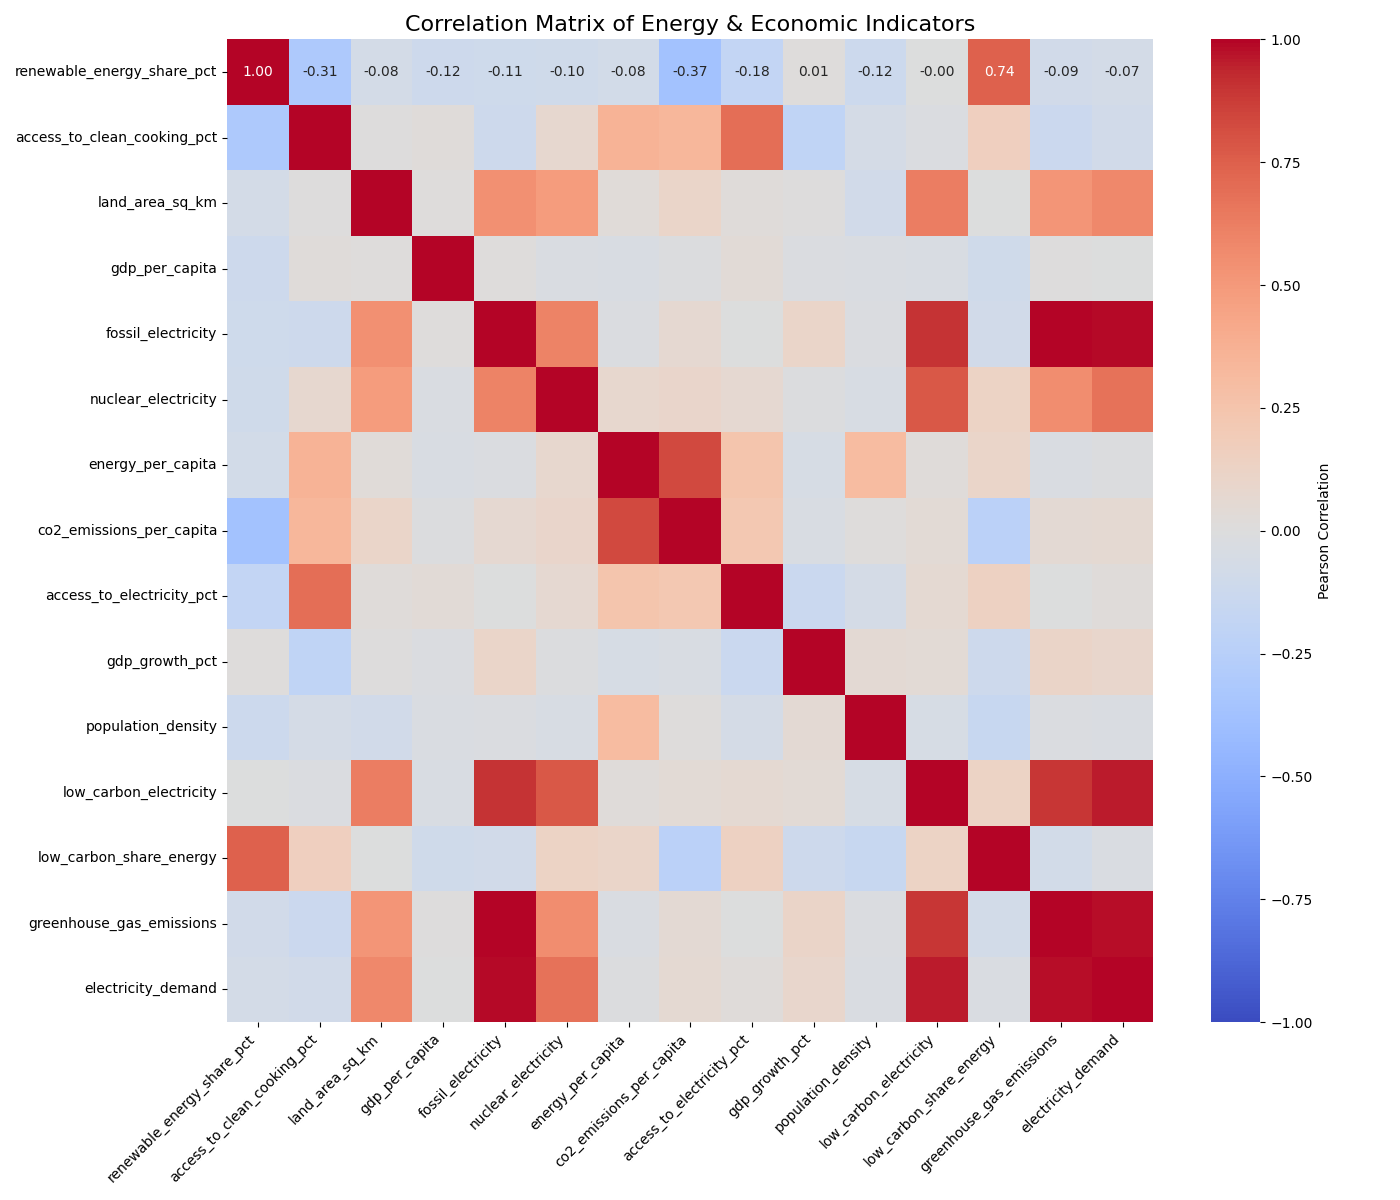
\includegraphics[width=0.75\textwidth]{Image/correlation_heatmap.png} 
    \caption{Correlation Heatmap of the Broad Independent Variables}
    \label{fig:heatmap}
\end{figure}

Beyond isolated variable distributions, the EDA evaluated the cross-sectional relationships between the predictors.
The Pearson correlation matrix (Figure \ref{fig:heatmap}) revealed severe structural multicollinearity among certain environmental and demand metrics.
For instance, absolute carbon dioxide emissions and overall electricity demand exhibited near-perfect collinearity with total fossil fuel generation.
These exploratory findings dictated the necessity of employing a strict 0.80 correlation threshold to drop collinear variables, thereby ensuring the mathematical stability of the inverted matrices in the final Fixed Effects panel models.

\subsection{Structural Variable Selection and Regime Identification}
To avoid endogenizing the specific policy levers intended for econometric testing, the pipeline deliberately split the variable usage.
For the Factor Analysis and clustering phase, the dataset was strictly restricted to six foundational macroeconomic and infrastructural traits: access to electricity, access to clean cooking, GDP per capita, GDP growth, energy per capita, and the baseline low-carbon energy share.
The rationale for this restriction was to ensure that the resulting regimes were defined purely by a nation's baseline developmental maturity, rather than being polluted by specific energy generation choices (such as nuclear or fossil fuel investments) which serve as the independent variables in the later regressions.

Prior to dimensionality reduction on these six variables, Bartlett's Test of Sphericity yielded a $p$-value of $2.71 \times 10^{-210}$, confirming sufficient correlation.
The Kaiser-Meyer-Olkin (KMO) measure produced an overall score of $0.665$, validating sampling adequacy.
The Factor Analysis successfully collapsed these six variables into three optimal latent dimensions (eigenvalues $>1$), isolating infrastructural maturity, environmental energy mix, and economic wealth.

\begin{figure}[hbt!]
    \centering
    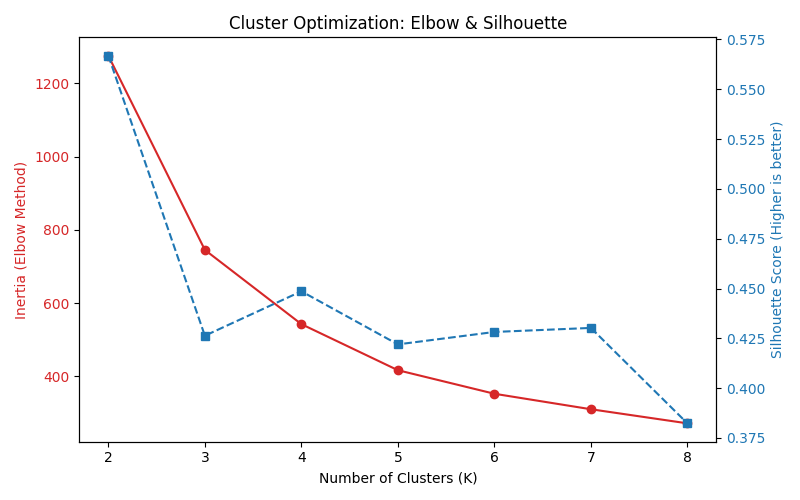
\includegraphics[width=0.7\textwidth]{Image/Cluster_Optimization.png}
    \caption{Silhouette Score Optimization for K-Means Clustering}
    \label{fig:cluster_opt}
\end{figure}

Following dimensionality reduction, the Silhouette Score optimization (Figure \ref{fig:cluster_opt}) recommended $K=2$ as the mathematically optimal number of regimes.
The $K$-Means algorithm successfully partitioned the data into:
\begin{itemize}
    \item \textbf{Cluster 0 (Developed / High-Energy Regime):} Characterized by absolute infrastructural maturity (100\% median access to electricity and clean cooking), massive energy consumption per capita (34,152 kWh), and a higher baseline low-carbon energy share (13.32\%).
    \item \textbf{Cluster 1 (Developing / High-Growth Regime):} Characterized by incomplete infrastructural access (92.0\% median access to electricity, and only 41.6\% access to clean cooking), high economic growth (6.34\%), and lower energy consumption per capita (4,220 kWh).
\end{itemize}

\subsection{Temporal Dynamics and Stationarity}
The Time Series Analyzer evaluated the renewable energy share over the 2012--2021 decade to understand the trajectory and inertia of the global transition.

\begin{figure}[hbt!]
    \centering
    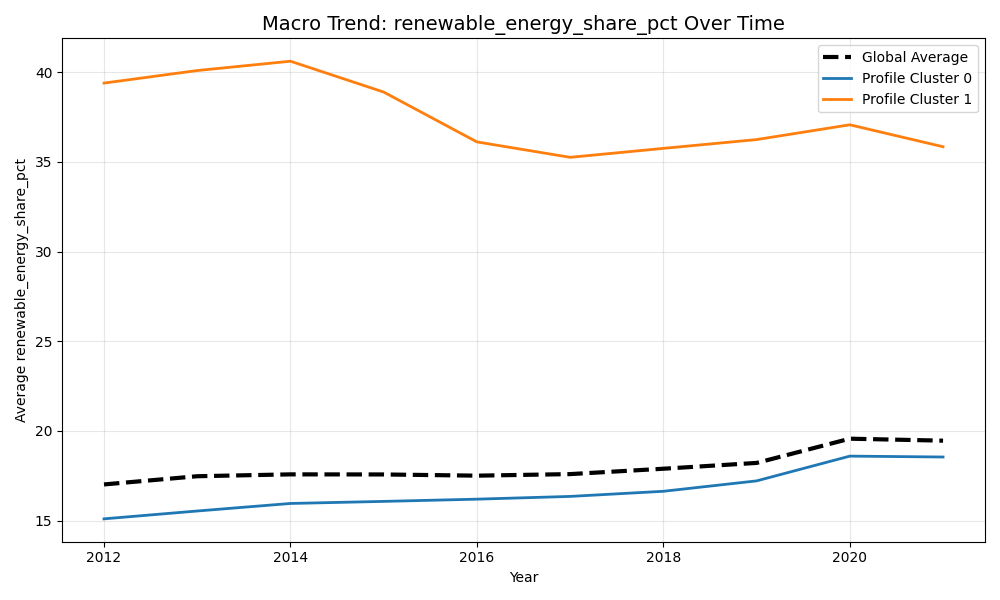
\includegraphics[width=0.7\textwidth]{Image/TSA_Macro_Trends.png}
    \caption{Macro Trend Analysis of Renewable Energy Share by Regime (2012-2021)}
    \label{fig:macro_trends}
\end{figure}

As shown in Figure \ref{fig:macro_trends}, both regimes exhibit upward trajectories, reflecting the global momentum of the post-Paris Agreement era.
However, the Augmented Dickey-Fuller (ADF) test yielded a test statistic of $0.4416$ ($p=0.9830$), definitively failing to reject the null hypothesis.
This confirms that renewable energy share is a non-stationary process possessing a significant time trend, mandating the inclusion of time-fixed effects in the final econometric models.
Furthermore, autocorrelation analysis confirmed severe path-dependency at Lag 1, indicating that a nation's energy mix is heavily dictated by its pre-existing physical infrastructure.

\subsection{Econometric Preparation and Fractional Estimates}
For the final econometric phase, the analytical approach shifted.
Rather than relying on the six restricted factors, the broader panel of 14 independent variables was reintroduced to test specific policy levers within the newly defined regimes.
To resolve the multicollinearity identified during the EDA, a strict 0.80 correlation threshold was enforced.
This automated processing systematically dropped highly collinear variables, such as total $CO_2$ emissions and absolute electricity demand, resulting in a robust, mathematically stable subset of 11 independent variables.

To isolate the macro-level drivers while respecting the bounded $0-100\%$ nature of the dependent variable, the Correlated Random Effects (CRE) Fractional Probit and the Log-Odds Transformed Fixed Effects models were executed on these 11 variables.
The comparative results are presented in Table \ref{tab:econometrics}.

\begin{table}[hbt!]
\centering
\caption{Econometric Estimates for Renewable Energy Adoption by Regime}
\label{tab:econometrics}
\resizebox{\textwidth}{!}{
\begin{tabular}{l cc | cc}
\toprule
 & \multicolumn{2}{c}{\textbf{Cluster 0: Developed Regime}} & \multicolumn{2}{c}{\textbf{Cluster 1: Developing Regime}} \\
\cmidrule(lr){2-3} \cmidrule(lr){4-5}
\textbf{Independent Variables} & \textbf{PW2008 (CRE Probit)} & \textbf{Ramalho2017 (Log-Odds)} & \textbf{PW2008 (CRE Probit)} & \textbf{Ramalho2017 (Log-Odds)} \\
\midrule
Access to Clean Cooking (\%) & $-0.6915^{***}$ & $-0.8691^{***}$ & $0.6050^{***}$ & $1.0763^{***}$ \\
Land Area (sq. km)          & $0.5142$        & $3.2100$        & $6.5223^{***}$ & $8.2908^{***}$ \\
GDP per Capita              & $0.2300^{***}$  & $0.4567^{***}$  & $-0.2308^{**}$ & $-0.2808$ \\
Fossil Electricity          & $-0.1825^{***}$ & $-0.2996^{***}$ & $-0.3385^{***}$ & $-0.4793^{***}$ \\
Nuclear Electricity         & $0.0024$        & $-0.0116$       & $0.0158^{*}$    & $0.0164$ \\
Energy per Capita           & $-0.2901^{**}$  & $-1.2761^{***}$ & $-0.0975^{**}$  & $-0.0886$ \\
Access to Electricity (\%)  & $0.5295$        & $-2.6162^{*}$   & $-0.0449$       & $-0.2700$ \\
GDP Growth (\%)             & $0.0005$        & $0.0003$        & $-0.0015$       & $0.0008$ \\
Population Density          & $0.3728$        & $0.3784$        & $-0.5307^{*}$   & $-0.7310$ \\
Low-Carbon Electricity      & $-0.0604$       & $0.6180^{***}$  & $-0.1206^{***}$ & $-0.1505^{*}$ \\
Low-Carbon Share of Energy  & $0.2750^{*}$    & $-0.0264$       & $0.0465^{***}$  & $0.0721^{**}$ \\
\midrule
\multicolumn{5}{l}{\footnotesize Significance levels: $^{***} p<0.01$, $^{**} p<0.05$, $^{*} p<0.10$.} \\
\multicolumn{5}{l}{\footnotesize Note: Mundlak country-mean controls were included in the PW2008 specification but are omitted from} \\
\multicolumn{5}{l}{\footnotesize this table for brevity. Magnitudes are not directly comparable across models due to varying link functions.} \\
\bottomrule
\end{tabular}
}
\end{table}

% ---------------------------------------------------------
\section{Discussion}
The empirical results of this study fundamentally validate the core hypothesis: the macroeconomic drivers of renewable energy adoption are highly heterogeneous and strictly dependent on a nation's developmental regime.
By mathematically partitioning the panel data into Developed (Cluster 0) and Developing (Cluster 1) profiles, the econometric models successfully exposed severe divergences in how policy levers operate—nuances that would have been entirely obscured by a traditional pooled global regression. 

\subsection{The Divergent Impact of Economic Wealth}
The relationship between economic capacity and renewable energy adoption splits sharply along regime lines.
In the Developed regime, absolute wealth (GDP per Capita) is a highly significant positive driver ($p < 0.01$).
This confirms that transitioning a legacy grid requires massive, centralized capital expenditure.
Wealthy nations possess the financial leverage necessary to subsidize renewable technology, absorb the premium of early-stage green infrastructure, and manage the economic fallout of decommissioning functional fossil-fuel assets. 

Conversely, in the Developing regime, economic capacity exhibits a negative elasticity.
This phenomenon aligns closely with the Environmental Kuznets Curve theory: rapidly industrializing nations often prioritize absolute economic growth and poverty reduction over environmental sustainability.
In these economies, capital is directed toward the fastest and cheapest available energy sources—historically coal and natural gas—to fuel industrial expansion, thereby suppressing the overall percentage share of renewables in their energy mix.

\subsection{Infrastructural Expansion vs. Saturation}
The most striking divergence between the two regimes lies in the impact of foundational infrastructure.
In Developing nations, \textit{Access to Clean Cooking} exhibits a highly significant, positive elasticity ($p < 0.01$) across both the Fractional Probit and Log-Odds models.
In these economies, shifting populations away from traditional, highly polluting biomass fuels toward modern electricity grids acts as a direct catalyst for renewable energy adoption, because new grid capacity in the modern era is increasingly fulfilled by cost-competitive solar and wind. 

In Developed nations—where 100\% baseline access is already universally achieved—the coefficient for \textit{Access to Clean Cooking} becomes strongly negative.
In this context, the variable acts as a proxy for highly energy-intensive, fully industrialized societies.
Similarly, \textit{Energy per Capita} exerts a significant negative drag in Developed nations.
This indicates that extreme energy consumption acts as a mathematical anchor; when total energy demand is extraordinarily high, adding renewable capacity barely impacts the percentage \textit{share} of the total mix, highlighting energy efficiency as a critical bottleneck for wealthy nations.

\subsection{Spatial Dynamics and Leapfrogging}
Geographic realities dictate transition strategies disproportionately.
In Developing nations, \textit{Land Area} is a massively significant, positive driver of renewable energy adoption ($p < 0.01$).
Utility-scale renewable infrastructure, particularly solar arrays and wind farms, requires vast spatial footprints compared to dense coal or nuclear plants.
For developing nations, possessing vast tracts of available land is a critical prerequisite for leapfrogging fossil fuels and scaling green grids.
In Developed nations, however, land area is statistically insignificant, likely due to older, denser grid infrastructures, administrative zoning barriers, and a higher reliance on distributed generation (e.g., rooftop solar) or offshore wind, which bypass domestic spatial constraints.

\subsection{The Universal Barrier: Fossil Fuel Lock-in}
Despite the stark developmental differences, one variable operated universally: \textit{Fossil Electricity} generation exerted a highly significant, negative drag on renewable energy adoption across all models and all clusters ($p < 0.01$).
This highlights the profound phenomenon of "carbon lock-in".
Regardless of whether a nation is wealthy or developing, the existence of an entrenched fossil fuel industry creates severe infrastructural, economic, and political inertia. 

Furthermore, the Time Series Analysis confirmed that the transition is highly path-dependent (Autocorrelation Lag 1) and that global convergence is failing, with the statistical gap between leading and lagging nations actively widening over the decade.

\subsection{Strategic Implications for Policymakers}
The deployment of these findings provides highly actionable, regime-specific intelligence for international financial institutions and policymakers:
\begin{itemize}
    \item \textbf{Policy Directives for Developing Regimes (Cluster 1):} International climate finance should not strictly focus on isolated technology subsidies. Because infrastructural access is a positive driver of renewables in this cluster, funds should be directed toward foundational grid modernization and electrification programs. By pairing basic electricity and clean cooking expansion with decentralized solar and wind micro-grids, these nations can bypass legacy fossil fuels. Additionally, policies must account for the spatial constraints of these nations, utilizing their vast land area for utility-scale deployment before carbon-intensive industrialization locks them into fossil fuels.
    \item \textbf{Policy Directives for Developed Regimes (Cluster 0):} The bottleneck for advanced economies is not a lack of grid infrastructure, but rather hyper-consumption and carbon lock-in. Policymakers must pivot away from merely subsidizing new green energy and actively implement aggressive demand-side reduction policies (improving energy efficiency). Most importantly, the universal negative drag of fossil fuels mathematically proves that adding renewables is insufficient; active, legislated phase-outs and carbon pricing mechanisms are required to force the decommissioning of legacy carbon assets.
\end{itemize}

% ---------------------------------------------------------
\section{Conclusions}

This study sought to resolve a critical limitation in contemporary macroeconomic energy research: the reliance on homogeneous models that prescribe uniform climate policies across inherently disparate nations.
Guided by the POST-DS methodology, the research employed a blended analytical framework—integrating unsupervised machine learning, temporal analysis, and fractional panel econometrics—to quantify the macro-level drivers of renewable energy adoption across the 2012--2021 decade.
By mathematically partitioning the global dataset into distinct Developed and Developing regimes, the models successfully captured the unobserved structural heterogeneity that traditional pooled global regressions obscure.

The empirical findings definitively prove that the transition to renewable energy is not driven by a universal set of socioeconomic levers.
In developing economies, foundational infrastructural expansion, such as access to clean cooking and modern electricity, and vast geographic land area serve as critical catalysts for leapfrogging legacy energy systems.
Conversely, in advanced economies, absolute economic wealth is required to overcome the immense capital costs of transitioning fully saturated, high-demand grids. However, despite these divergent structural profiles, the analysis identified carbon lock-in—represented by entrenched fossil fuel electricity generation—as a universal mathematical barrier that actively suppresses the renewable energy share across all global contexts. 

Ultimately, this research provides highly actionable, regime-specific intelligence for global policymakers and international financial institutions.
The results emphasize that international climate finance cannot rely exclusively on generic technology subsidies.
Instead, capital must be strategically deployed according to a nation's specific developmental bottleneck—prioritizing basic grid modernization in emerging markets while enforcing aggressive fossil-fuel decommissioning and demand-side energy efficiency in advanced economies.
By embracing this targeted, data-driven framework, global institutions can more effectively accelerate the international transition toward a sustainable energy future.

\newpage
% Print the bibliography in APA format
\printbibliography

\end{document}
